\documentclass{article}
\usepackage{hyperref}
\usepackage{graphicx}
\usepackage{amsmath}
\usepackage{caption}
\graphicspath{ {images/} }

\begin{document}
\section{Introduction}

%% What sympy is, where to download etc.
%%
%% List other major CASs.
%%
%% Why SymPy.

SymPy is a full featured computer algebra system (CAS) written in the Python
programming language. It is open source, licensed under the extremely
permissive 3-clause BSD license, which allows anyone to reuse SymPy or its source code,
even for commercial purposes. SymPy was started by Ond\v{r}ej \v{C}ert\'{\i}k
in 2005, and it has since grown into a large open source project, with over
500 contributors.
% citation?

SymPy is written entirely in the Python programming language,
% cite Python?
which is also the language used to interact with it, both programmatically and
interactively. Python is a popular dynamically typed programming language that
has a focus on ease of use and readability. Unlike many CASs, SymPy does not
invent its own programming language. We rather take the approach that Python
is already a well-designed programming language, built by expert language
designers, something which the majority of SymPy developers are not. Python is
also a very popular language for scientific computing and data science, with a
wide range of useful libraries.
% Cite numpy, scipy, pandas
% We could also cite
% https://stackoverflow.com/research/developer-survey-2016#most-popular-technologies-per-occupation

SymPy is designed with a strong focus that it be usable as a library. This
means that extensibility is important in its API design. This is also one of
the reasons SymPy makes no attempt to extend the Python language itself. The
goal is for users of SymPy to be able to import SymPy alongside other Python
libraries in their workflow, whether that is an interactive workflow or
programmatic use as part of a larger library. This does have some downsides;
for instance, unlike many popular CASs, all variables in SymPy must be defined
before they are used (Python does not provide a mechanism to automatically
declare variables). This is a minor inconvenience for interactive use, but we
consider it to be good practice for any reproducible work, and it aligns with
the philosophy of Python, ``explicit is better than implicit.''
% cite https://www.python.org/dev/peps/pep-0020/

SymPy does not have a built in graphical user interface (GUI), however, when
used in the Jupyter Notebook
% citation
SymPy expressions will pretty print using MathJax.
% citation


\section{Architecture}


%% I volunteer to write this section. --Aaron
%%
%% Representing symbolic expressions using Python objects

\subsection{The Core}

Every symbolic expression in SymPy is an instance of a Python class.
Expressions are represented by expression trees. The operators are represented
by the type of an expression and the child nodes are stored in the
\texttt{args} attribute. A leaf node in the expression tree has an empty
\texttt{args}.
The \texttt{args} attribute is provided by the class \texttt{Basic},
which is a superclass of all SymPy objects and
provides common methods to all SymPy tree-elements.
For example, take the expression $xy + 2$.

\begin{verbatim}
>>> from sympy import *
>>> x, y = symbols('x y')
>>> expr = x*y + 2
\end{verbatim}

The expression \texttt{expr} is an addition, so it is of type \texttt{Add}. The child
nodes of \texttt{expr} are \texttt{x*y} and \texttt{2}.

\begin{verbatim}
>>> type(expr)
<class 'sympy.core.add.Add'>
>>> expr.args
(2, x*y)
\end{verbatim}

We can dig further into the expression tree to see the full expression. For
example, the first child node, given by \texttt{expr.args[0]} is
\texttt{2}. Its class is \texttt{Integer}, and it has empty \texttt{args},
indicating that it is a leaf node.

\begin{verbatim}
>>> expr.args[0]
2
>>> type(expr.args[0])
<class 'sympy.core.numbers.Integer'>
>>> expr.args[0].args
()
\end{verbatim}

The function \texttt{srepr} gives a string representing a valid Python code,
containing all the nested class constructor calls to create the given expression.

\begin{verbatim}
>>> srepr(expr)
"Add(Mul(Symbol('x'), Symbol('y')), Integer(2))"
\end{verbatim}

Every SymPy expression satisfies a key invariant, namely,
\texttt{expr.func(*expr.args) == expr}. This means that expressions are
rebuildable from their \texttt{args}~\footnote{\texttt{expr.func} is used
  instead of \texttt{type(expr)} to allow the function of an expression to be
  distinct from its actual Python class. In most cases the two are the same.}.
Here, we note that in SymPy, the \texttt{==} operator represents exact
structural equality, not mathematical equality. This allows one to test if any
two expressions are equal to one another as expression trees.

Python allows classes to overload operators. The Python interpreter translates
the above \texttt{x*y + 2} to, roughly,
\verb|(x.__mul__(y)).__add__(2)|. \texttt{x} and \texttt{y}, returned from
the \texttt{symbols} function, are \texttt{Symbol} instances. The \texttt{2}
in the expression is processed by Python as a literal, and is stored as
Python's builtin \texttt{int} type. When \texttt{2} is called by the
\verb|__add__| method, it is converted to the SymPy type \texttt{Integer(2)}. In
this way, SymPy expressions can be built in the natural way using Python
operators and numeric literals.

One must be careful in one particular instance. Python does not have a builtin
rational literal type. Given a fraction of integers such as \texttt{1/2},
Python will perform floating point division and produce
\texttt{0.5}~\footnote{This is the behavior in Python 3. In Python 2,
  \texttt{1/2} will perform integer division and produce \texttt{0}, unless
  one uses \texttt{from \_\_future\_\_ import division}.}. Python uses eager
evaluation, so expressions like \texttt{x + 1/2} will produce \texttt{x +
  0.5}, and by the time any SymPy function sees the \texttt{1/2} it has
already been converted to \texttt{0.5} by Python. However, for a CAS like
SymPy, one typically wants to work with exact rational numbers whenever
possible. Working around this is simple, however:  one can wrap one of the
integers with \texttt{Integer}, like \texttt{x + Integer(1)/2}, or using
\texttt{x + Rational(1, 2)}. SymPy provides a function \texttt{S} which can be
used to convert objects to SymPy types with minimal typing, such as \texttt{x
  + S(1)/2}. This gotcha is a small downside to using Python directly instead
of a custom domain specific language (DSL), and we consider it to be worth it
for the advantages listed above.

%%
%% Assumptions
\subsection{Assumptions}

An important feature of the SymPy core is the assumptions system. The
assumptions system allows users to specify that symbols have certain common
mathematical properties, such as being positive, imaginary, or integer. SymPy
is careful to never perform simplifications on an expression unless the
assumptions allow them. For instance, the identity $\sqrt{x^2} = x$ holds if
$x$ is nonnegative ($x\ge 0$). If $x$ is real, the identity $\sqrt{x^2}=|x|$
holds. However, for general complex $x$, no such identity holds.

By default, SymPy performs all calculations assuming that variables are
complex valued. This assumption makes it easier to treat mathematical problems
in full generality.

\begin{verbatim}
>>> x = Symbol('x')
>>> sqrt(x**2)
sqrt(x**2)
\end{verbatim}

By assuming symbols are complex by default, SymPy avoids performing
mathematically invalid operations. However, in many cases users will wish to
simplify expressions containing terms like $\sqrt{x^2}$.

Assumptions are set on \texttt{Symbol} objects when they are created. For
instance \texttt{Symbol('x', positive=True)} will create a symbol named
\texttt{x} that is assumed to be positive.

\begin{verbatim}
>>> x = Symbol('x', positive=True)
>>> sqrt(x**2)
x
\end{verbatim}

Some common assumptions that SymPy allows are \texttt{positive},
\texttt{negative}, \texttt{real}, \texttt{nonpositive}, \texttt{nonnegative},
\texttt{real}, \texttt{integer}, and \texttt{commutative}~\footnote{If $A$ and
  $B$ are Symbols created with \texttt{commutative=False} then SymPy will keep
  $A\cdot B$ and $B\cdot A$ distinct.}. Assumptions on any object can be checked with the
\verb|is_|\texttt{\textit{assumption}} attributes, like \verb|x.is_positive|.

Assumptions are only needed to restrict a domain so that certain
simplifications can be performed. It is not required to make the domain match
the input of a function. For instance, one can create the object
$\sum_{n=0}^m f(n)$ as \texttt{Sum(f(n), (n, 0, m))} without setting
\texttt{integer=True} when creating the Symbol object \texttt{n}.

The assumptions system additionally has deductive capabilities. The
assumptions use a three-valued logic using the Python builtin objects
\texttt{True}, \texttt{False}, and \texttt{None}. \texttt{None} represents the
``unknown'' case. This could mean that the given assumption could be either
true or false under the given information, for instance,
\verb|Symbol('x', real=True).is_positive| will give \texttt{None} because a real
symbol might be positive or it might not. It could also mean not enough is
implemented to compute the given fact, for instance,
\verb|(pi + E).is_irrational| gives \texttt{None}, because SymPy does not know
how to determine if $\pi + e$ is rational or irrational, indeed, it is an open
problem in mathematics. % ref?


Basic implications between the facts are used to deduce assumptions. For
instance, the assumptions system knows that being an integer implies being
rational, so \verb|Symbol('x', integer=True).is_rational| returns
\texttt{True}. Furthermore, expressions compute the assumptions on themselves
based on the assumptions of their arguments. For instance, if \texttt{x} and
\texttt{y} are both created with \texttt{positive=True}, then \verb|(x + y).is_positive|
will be \texttt{True}.

SymPy also has an experimental assumptions system where facts are stored
separate from objects, and deductions are made with a SAT solver. We will not
discuss this system here.

%%
%% Extensibility
\subsection{Extensibility}

Extensibility is an important feature for SymPy. Because the same language,
Python, is used both for the internal implementation and the external usage by
users, all the extensibility capabilities available to users are also used by
functions that are part of SymPy.

The typical way to create a custom SymPy object is to subclass an existing
SymPy class, generally either \texttt{Basic}, \texttt{Expr}, or
\texttt{Function}. All SymPy classes used for expression trees~\footnote{Some
  internal classes, such as those used in the polynomial module, do not follow
  this rule.} should be subclasses of the base class
\texttt{Basic}, which defines some basic methods for symbolic expression
trees. \texttt{Expr} is the subclass for mathematical expressions that can be
added and multiplied together. Instances of \texttt{Expr} are typically
complex numbers, but may also include other ``rings'' like matrix expressions.
Not all SymPy classes are \texttt{Expr}. For instance, logic expressions, such
as \texttt{And(x, y)} are \texttt{Basic} but not \texttt{Expr}.

The \texttt{Function} class is a subclass of \texttt{Expr} which makes it
easier to define mathematical functions called with arguments. This includes
named functions like $\sin(x)$ and $\log(x)$ as well as undefined functions
like $f(x)$. Subclasses of \texttt{Function} should define a
class method \texttt{eval}, which returns values for which the function should
be automatically evaluated, and \texttt{None} for arguments that shouldn't be
automatically evaluated.

The behavior of classes in SymPy with various other SymPy functions is defined
by defining a relevant \verb|_eval_|\texttt{\textit{*}} method on the class. For instance, an
object can tell SymPy's \texttt{diff} function how to take the derivative of
itself by defining the \verb|_eval_derivative(self, x)| method. The most
common \verb|_eval_|\texttt{\textit{*}} methods relate to the assumptions.
\verb|_eval_is_|\texttt{\textit{assumption}} defines the assumptions for
\textit{assumption}.

Here is a stripped down version of the gamma function $\Gamma(x)$ from SymPy,
which evaluates itself on positive integer arguments, has the positive and
real assumptions defined, can be rewritten in terms of factorial with
\texttt{gamma(x).rewrite(factorial)}, and can be differentiated.
\texttt{fdiff} is a convenience method for subclasses of \texttt{Function}.
\texttt{fdiff} returns the derivative of the function without worrying about
the chain rule. \texttt{self.func} is used throughout instead of referencing
\texttt{gamma} explicitly so that potential subclasses of \texttt{gamma} can
reuse the methods.

\begin{verbatim}
from sympy import Integer, Function, floor, factorial, polygamma

class gamma(Function)
    @classmethod
    def eval(cls, arg):
        if isinstance(arg, Integer) and arg.is_positive:
            return factorial(arg - 1)

    def _eval_is_real(self):
        x = self.args[0]
        # noninteger means real and not integer
        if x.is_positive or x.is_noninteger:
            return True

    def _eval_is_positive(self):
        x = self.args[0]
        if x.is_positive:
            return True
        elif x.is_noninteger:
            return floor(x).is_even

    def _eval_rewrite_as_factorial(self, z):
        return factorial(z - 1)

    def fdiff(self, argindex=1):
        from sympy.core.function import ArgumentIndexError
        if argindex == 1:
            return self.func(self.args[0])*polygamma(0, self.args[0])
        else:
            raise ArgumentIndexError(self, argindex)
\end{verbatim}

The actual gamma function defined in SymPy has much more implemented than
this, such as evaluation at rational points and series expansion.


\section{Algorithms}

%% Description of some algorithms (example: integration with Risch, Meijer G, Gruntz, polys)
%%
%% Description of numerics/mpmath (Fredrik)

% A description of some of the algorithms in SymPy. The list is not
% exhaustive.

% The sections here are preliminary. We may end up needing to cut some of
% this.

% XXX: Perhaps this should just be integrated into the features section.

\subsection{Numerics}

\subsection{Polynomials}

\subsection{The Risch Algorithm}
% Also the Meijer-G algorithm, if someone can write about it

\subsection{The Gruntz Algorithm}

The limit module implements the Gruntz algorithm
\cite{gruntz1996computing}.

Examples:
\begin{verbatim}
In [1]: limit(sin(x)/x, x, 0)
Out[1]: 1

In [2]: limit((2*E**((1-cos(x))/sin(x))-1)**(sinh(x)/atan(x)**2), x, 0)
Out[2]: E
\end{verbatim}

\subsubsection{Details}

We first define comparability classes by calculating $L$:
\begin{equation}
L\equiv \lim_{x\to\infty} {\log |f(x)| \over \log |g(x)|}
\end{equation}
And then we define the $<$, $>$ and $\sim$ operations as follows: $f>g$ when
$L=\pm\infty$ ($f$ is more rapidly varying than $g$, i.e. $f$ goes to $\infty$
or $0$ faster than $g$, $f$ is greater than any power of $g$), $f<g$ when $L=0$
($f$ is less rapidly varying than $g$) and $f\sim g$ when $L\neq 0,\pm\infty$
(both $f$ and $g$ are bounded from above and below by suitable integral powers
of the other).

Examples:
$$2 < x < e^x < e^{x^2} < e^{e^x}$$
$$2\sim 3\sim -5$$
$$x\sim x^2\sim x^3\sim {1\over x}\sim x^m\sim -x$$
$$e^x\sim e^{-x}\sim e^{2x}\sim e^{x+e^{-x}}$$
$$f(x)\sim{1\over f(x)}$$

The Gruntz algorithm, on an example:
$$f(x) = e^{x+2e^{-x}} - e^x + {1\over x}$$
$$\lim_{x\to\infty} f(x) = ?$$

Strategy:
mrv set: the set of most rapidly varying subexpressions
$\{e^x, e^{-x}, e^{x+2e^{-x}}\}$, the same comparability class
Take an item $\omega$ from mrv, converging to 0 at infinity. Here
$\omega=e^{-x}$. If not present in the mrv set, use the relation
$f(x)\sim {1\over f(x)}$.

Rewrite the mrv set using $\omega$: $\{{1\over\omega}, \omega,
{1\over\omega}e^{2\omega}\}$, substitute back into $f(x)$ and expand in
$\omega$:
$$f(x) = {1\over x}-{1\over\omega}+{1\over\omega}e^{2\omega}
    = 2+{1\over x} + 2\omega + O(\omega^2)$$

The core idea of the algorithm: $\omega$ is from the mrv set, so in the limit
$\omega\to0$:
$$f(x) = {1\over x}-{1\over\omega}+{1\over\omega}e^{2\omega}
    = 2+{1\over x} + 2\omega + O(\omega^2)
    \to 2 + {1\over x}$$

We iterate until we get just a number, the final limit. Gruntz proved this
algorithm always works and converges in his Ph.D. thesis
\cite{gruntz1996computing}.

Generally:
$$ f(x) = \underbrace{O\left({1\over \omega^3}\right)}_\infty
    + \underbrace{C_{-2}(x)\over \omega^2}_\infty
    + \underbrace{C_{-1}(x)\over \omega}_\infty
    + {C_{0}(x)}
    + \underbrace{C_{1}(x)\omega}_0
    + \underbrace{O(\omega^2)}_0
$$
we look at the lowest power of $\omega$. The limit is one of: $0$,
$\lim_{x\to\infty} C_0(x)$, $\infty$.

\subsection{Logic}

\subsection{Other}


\section{Features}

%% List of Features and how to use
%%
%% Quick overview of the main modules, what it can do and so on. It should probably provide examples how to use sympy.
%%
%% See also the supplement (below)

% Features to discuss in-depth:

% Basic operations (the core)
\subsection{Basic Operations}

\input{features_basic_operations}

\subsection{Calculus}

% Solvers (regular equations, maybe also mention other types of solvers like ODEs/recurrence/Diophantine)
\subsection{Solvers}
%% Solvers in SymPy


SymPy has a solvers module to solve equations symbolically. There are two
submodules to solve algebraic equations in SymPy, referred to as old solve
i.e. \texttt{solve} and new solve i.e. \texttt{solveset}. Solveset is
introduced with several design changes with respect to old \texttt{solve} to
resolve the issues with old \texttt{solve}, for example old \texttt{solve}'s
input API has many flags which are not needed and they make it hard for the
user and the developers to work on solvers. In contrast to old solve, the
\texttt{solveset} has a clean input API, It only asks for the much needed
information from the user, following are the function signatures of old and new
solve:

\begin{verbatim}
solve(f, *symbols, **flags)  # old solve
solveset(f, symbol, domain)  # new solve
\end{verbatim}

The old \texttt{solve} has an inconsistent output API for various types of
inputs, whereas the \texttt{solveset} has a canonical output API which is
achieved using sets. It can consistently return various types of solutions.

\begin{itemize}
\item Single solution
\end{itemize}
\begin{verbatim}
>>> solveset(x - 1)
>>> {1}
\end{verbatim}

\begin{itemize}
\item Finite set of solution, quadratic equation
\end{itemize}
\begin{verbatim}
>>> solveset(x**2 - pi**2, x)
{-pi, pi}
\end{verbatim}

\begin{itemize}
\item No Solution
\end{itemize}
\begin{verbatim}
>>> solveset(1, x)
EmptySet()
\end{verbatim}

\begin{itemize}
\item Interval of solution
\end{itemize}
\begin{verbatim}
>>> solveset(x**2 - 3 > 0, x, domain=S.Reals)
(-oo, -sqrt(3)) U (sqrt(3), oo)
\end{verbatim}

\begin{itemize}
\item Infinitely many solutions
\end{itemize}
\begin{verbatim}
>>> solveset(sin(x) - 1, x, domain=S.Reals)
ImageSet(Lambda(_n, 2*_n*pi + pi/2), Integers())
>>> solveset(x - x, x, domain=S.Reals)
(-oo, oo)
>>> solveset(x - x, x, domain=S.Complexes)
S.Complexes
\end{verbatim}

\begin{itemize}
\item Linear system: finite and infinite solution for determined, under
determined and over determined problems.
\end{itemize}
\begin{verbatim}
>>> A = Matrix([[1, 2, 3], [4, 5, 6], [7, 8, 10]])
>>> b = Matrix([3, 6, 9])
>>> linsolve((A, b), x, y, z)
{(−1,2,0)}
>>> linsolve(Matrix(([1, 1, 1, 1], [1, 1, 2, 3])), (x, y, z))
{(-y - 1, y, 2)}
\end{verbatim}

The new solve i.e. \textbf{solveset} is under active development and is a
planned replacement for \textbf{solve}, Hence there are some features which are
implemented in solve and is not yet implemented in solveset. The table below
show the current state of old and new solve.

\hfill

\begin{tabular}{ |p{4cm}|p{3cm}|p{3cm}|  }
\hline
\multicolumn{3}{|c|}{Solveset vs Solve} \\
\hline
Feature& solve &solveset \\
\hline
Consistent Output API & No & Yes \\
Consistent Input API & No & Yes \\
Univariate & Yes & Yes\\
Linear System& Yes & Yes (linsolve) \\
Non Linear System& Yes & Not yet \\
Transcendental& Yes & Not yet \\
\hline
\end{tabular}

\hfill \break

Below are some of the examples of old \textbf{solve} :

\begin{itemize}
\item Non Linear (multivariate) System of Equation: Intersection of a circle
and a parabola.
\end{itemize}
\begin{verbatim}
>>> solve([x**2 + y**2 - 16, 4*x - y**2 + 6], x, y)
[(-2 + sqrt(14), -sqrt(-2 + 4*sqrt(14))),
 (-2 + sqrt(14), sqrt(-2 + 4*sqrt(14))),
 (-sqrt(14) - 2, -I*sqrt(2 + 4*sqrt(14))),
 (-sqrt(14) - 2, I*sqrt(2 + 4*sqrt(14)))]
\end{verbatim}

\begin{itemize}
\item Transcendental Equation
\end{itemize}
\begin{verbatim}
>>> solve(x + log(x))**2 - 5*(x + log(x)) + 6, x)
[LambertW(exp(2)), LambertW(exp(3))]
>>> solve(x**3 + exp(x))
[-3*LambertW((-1)**(2/3)/3)]
\end{verbatim}


% Matrices (worth including to stress that they are symbolic)
\subsection{Matrices}

% Physics module (some sampling, to show that it is there)
\subsection{Physics}

% Logic module
\subsection{Logic}

SymPy supports construction and manipulation of boolean expressions
through the \texttt{logic} module. SymPy symbols can be used as 
propositional variables and also be substituted as \texttt{True} 
or \texttt{False}. A good number of manipulation features for boolean 
expressions have been implemented in the \texttt{logic} module.

\subsubsection{Constructing boolean expressions}

A boolean variable can be declared as a SymPy symbol. Python
operators \&, \textbar  and \textasciitilde are overloaded for logical \texttt{And}, 
\texttt{Or} and \texttt{negate}. Several others like \texttt{Xor},
\texttt{Implies} can be constructed with \^{}, \textgreater\textgreater respectively.  
The above are just a shorthand, expressions can also be constructed
by directly calling \texttt{And()}, \texttt{Or()}, \texttt{Not()},
\texttt{Xor()}, \texttt{Nand()}, \texttt{Nor()}, etc.
The boolean symbols can also be substituted \texttt{True} or \texttt{False}

\begin{verbatim}
>>> e = (x & y) | z
>>> e.subs({x: True, y: True, z: False})
True
\end{verbatim}

\subsubsection{CNF and DNF}

Any boolean expression can be converted to conjunctive normal 
form, disjunctive normal form and negation normal form. The 
API also permits to check if a boolean expression is in any 
of the above mentioned forms.

\begin{verbatim}
>>> to_cnf((A & B) | C)
And(Or(A, C), Or(B, C))
>>> to_dnf(A & (B | C))
Or(And(A, B), And(A, C))
>>> is_cnf((x | y) & z)
True
>>> is_dnf((x & y) | z) 
True
\end{verbatim}

\subsubsection{Simplification and Equivalence}

The module supports simplification of given boolean expression
by making deductions on it. Equivalence of two expressions can
also be checked. If so, it is possible to return the mapping of 
variables of two expressions so as to represent the 
same logical behaviour.

\begin{verbatim}
>>> e = a & (~a | ~b) & (a | c)
>>> simplify(e)
And(Not(b), a)
>>> e1 = a & (b | c)
>>> e2 = (x & y) | (x & z)
>>> bool_map(e1, e2)
(And(Or(b, c), a), {b: y, a: x, c: z})
\end{verbatim}

\subsubsection{SAT solving}

The module also supports satisfiability checking of a given
boolean expression. If satisfiable, it is possible to return 
a model for which the expression is satisfiable. The API also
supports returning all possible models. The SAT solver has 
a clause learning DPLL algorithm implemented with watch 
literal scheme and VSIDS heuristic\cite{moskewicz2008method}.

\begin{verbatim}
>>> satisfiable(a & (~a | b) & (~b | c) & ~c)
False
>>> satisfiable(a & (~a | b) & (~b | c) & c)
{b: True, a: True, c: True}
\end{verbatim}


% Features to list, but not discuss in-depth:

% discrete math, concrete math, plotting, geometry, statistics, polys,
% combinatorics/group theory, code generation, tensors, lie algebras,
% cryptography, category theory, special functions, sets, matrix expressions,
% series, or vectors.
\subsection{Other features}


\section{Other Projects that use SymPy}

\subsection{SymPy Gamma}\label{sympy-gamma}

SymPy Gamma is a simple web application that runs on Google App Engine. 
It executes and displays the results of SymPy expressions as well as
additional related computations, in a fashion similar to that of
Wolfram\textbar{}Alpha. For instance, entering an integer will display
its prime factors, digits in the base-10 expansion, and a factorization
diagram. Entering a function will display its docstring; in general,
entering an arbitrary expression will display its derivative, integral,
series expansion, plot, and roots.

SymPy Gamma also has several additional features than just computing the
results using SymPy.

\begin{itemize}
\item
  It displays integration steps, differentiation steps in detail, which
  can be viewed in Figure \ref{fig:integralsteps}:\par
\begin{minipage}{\textwidth}
    \centering
    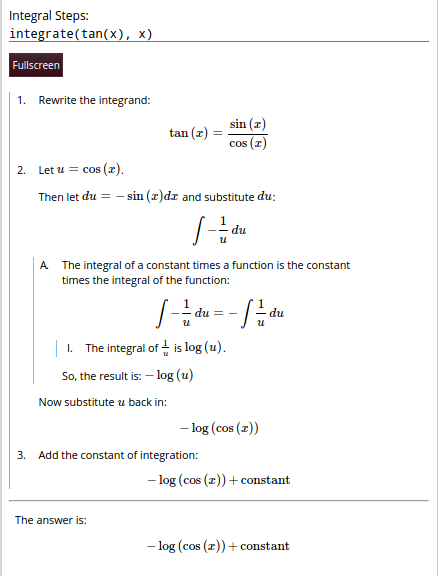
\includegraphics[width=0.7\textwidth]{integral_steps.png}
    \captionof{figure}{Integral steps of $\tan (x)$}
    \label{fig:integralsteps}
\end{minipage}
\item
  It also displays the factor tree diagrams for different numbers.
\item
  SymPy Gamma also saves user search queries, and offers many such 
  similar features for free, which Wolfram\textbar{}Alpha only offers 
  to its paid users.
\end{itemize}
Every input query from the user on SymPy Gamma is first, parsed by its
own parser, which handles several different forms of function names,
which SymPy as a library doesn't support. For instance, SymPy Gamma
supports queries like \texttt{sin\ x}, whereas SymPy doesn't support
this, and supports only \texttt{sin(x)}.

This parser converts the input query to the equivalent SymPy readable 
code, which is then eventually processed by SymPy and the result is 
finally formatted in LaTeX and displayed on the SymPy Gamma web-application.

\subsection{SymPy Live}\label{sympy-live}

SymPy Live is an online Python shell, which runs on Google
App Engine, that executes SymPy code. It is integrated in the SymPy
documentation examples, located at this \href{http://docs.sympy.org/latest/index.html}{link}.

This is accomplished by providing a HTML/JavaScript GUI for entering
source code and visualization of output, and a server part which
evaluates the requested source code. It's an interactive AJAX shell,
that runs SymPy code using Python on the server.
\newline
Certain Features of SymPy Live-:

\begin{itemize}
\item
  It supports the exact same syntax as SymPy, hence it can be used
  easily, to test for outputs of various SymPy expressions.
\item
  It can be run as a standalone app or in an existing app as an
  admin-only handler, and can also be used for system administration
  tasks, as an interactive way to try out APIs, or as a debugging aid
  during development.
\item
  It can also be used to plot figures (\href{http://live.sympy.org/?evaluate=from\%20sympy\%20import\%20symbols\%0Afrom\%20sympy.plotting\%20import\%20textplot\%0Ax\%20\%3D\%20symbols(\%27x\%27)\%0Atextplot(x**2\%2C0\%2C5)\%0A\%23--\%0A}{link}), 
  and execute all kinds of expressions that SymPy can evaluate.
\item
SymPy Live also formats the output in LaTeX for pretty-printing the
output.
\end{itemize}

\section{Comparison with other CAS}


\subsection{Mathematica}

Wolfram Mathematica is a popular proprietary CAS.
It features highly advanced algorithms.
Mathematica has a core implemented in C++~\cite{Wolfram2016}
which interprets its own programming language (know as Wolfram language).

% M-expressions

Analogously to Lisp's S-expressions,
Mathematica uses its own style of M-expressions,
which are arrays of either atoms or other M-expression.
The first element of the expression identifies the type of the expression
and is indexed by zero, whereas the first argument is indexed by one.
Notice that SymPy expression arguments are stored in a Python tuple
(that is, an immutable array),
while the expression type is identified by the type of the object storing the
expression.

% Attributes

Mathematica can associate attributes to its atoms.

% Expression mutability

Unlike SymPy, Mathematica's expressions are mutable,
that is one can change parts of the expression tree without the need of
creating a new object.
The reactivity of Mathematica allows for a lazy updating of any references
to that data structure.

% * comparison with Mathematica: commutativity, associative expressions, one-identity. Advantage of SymPy: multiplicative commutativity defined on symbols.
% Products and commutativity

Products in Mathematica are determined by some builtin node types,
such as \texttt{Times}, \texttt{Dot}, and others.
\texttt{Times} is overloaded by the * operator,
and is always meant to represent a commutative operator.
The other notable product is \texttt{Dot}, overloaded by the . operator.
This product represents matrix multiplication,
it is not commutative.
SymPy uses the same node for both scalar and matrix multiplication,
the only exception being with abstract matrix symbols.
Unlike Mathematica, SymPy determines commutativity with respect to
multiplication from the factor's expression type.
Mathematica puts the \texttt{Orderless} attribute on the expression
type.

% Associative expressions.

Regarding associative expressions,
SymPy handles associativity by making associative expressions inherit the
class \texttt{AssocOp},
while Mathematica specifies the \texttt{Flat}\cite{WolframRefFlat} attribute on the expression type.

% One identity


% Pattern matching

Mathematica relies heavily on pattern matching:
even the so-called equivalent of function declaration is in reality
the definition of a pattern matching generating an expression tree transformation
on input expressions.
%
Mathematica's pattern matching is sensitive to associative\cite{WolframRefFlat}, commutative\cite{WolframRefOrderless},
and one-identity\cite{WolframRefOneIdentity} properties of its expression tree nodes\cite{WolframRefFlatAndOrderlessFunctions}.
%
SymPy has various ways to perform pattern matching.
All of them play a lesser role in the CAS than in Mathematica.
looks less mature than Mathematica's,

%% TODO list:
% * comparison with Mathematica: MatrixExp, product not always commutative, type inheritance (polymorphism) and advantage in unifying the product symbol * for symbols and matrices, pattern matching vs. single dispatch.

% Type inheritance and polymorphism

Unlike SymPy, Mathematica does not support type inheritance or polymorphism\cite{Fateman1992}.
% cite examples of class inheritance in SymPy:
%
SymPy relies heavily on class inheritance, but for the most part,
class inheritance is used to make sure that SymPy objects inherit the proper
methods and implement the basic hashing system.
Associativity of expressions can be achieved by inheriting the class \texttt{AssocOp},
which may appear a more cumbersome operation than Mathematica's attribute setting.
%There are also cases where inheritance is used to extend the mathematical meaning of an expression.

% Matrices

Matrices in SymPy are types on their own.
In Mathematica, nested lists are interpreted as matrices whenever the sublists
have the same length.
The main difference to SymPy is that ordinary operators and functions
do not get generalized the same way as used in traditional mathematics.
Using the standard multiplication in Mathematica performs an elementwise
product, this is compatible with Mathematica's convention of commutativity of
\texttt{Times} nodes.
Matrix product is expressed by the \textit{dot} operator,
or the \texttt{Dot} node.
The same is true for the other operators, and even functions,
most notably calling the exponential function \texttt{Exp} on a matrix
returns an elementwise exponentiation of its elements.
The real matrix exponentiationl is available through the \texttt{MatrixExp}
function.

% * comparison with Mathematica: avoid misspelling variables through forced declaration (check that you can't do it in Mathematica).
% * evaluate=False vs HoldForm

Unevaluated expressions can be achieved in various ways,
most commonly with the \texttt{HoldForm} or \texttt{Hold} nodes,
that block the evaluation of subnodes by the parser.
Note that such a node cannot be expressed in Python, because of greedy evaluation.
Whenever needed in SymPy, it is necessary to add the parameter \texttt{evaluate=False}
to all subnodes, or put the input expression in a string.

% * comparison with Mathematica: == is structural equality, not

The operator == returns a boolean whenever it is able to immediately evaluate
the truthness of the equality, otherwise it returns an \texttt{Equal} expression.
In SymPy == means structural equality and is always guaranteed to return a
boolean expression.
To express an equality in SymPy it is necessary to explicitly construct the
\texttt{Equality} class.

% * comparison with Mathematica: polynomial module.
% * comparison with Mathematica: space is product, ** vs ^

SymPy, in accordance with Python and unlike the usual programming convention,
uses ** to express the power operator, while Mathematica uses the more
common \verb|^|.

% * comparison with Mathematica: ( ) is Sequence, functions are generally uppercase.
% * comparsion with Mathematica: table of comparison?
% * comparison with Mathematica: Wolfram language has loads of operator overloading, functional paradigm.


\section{Conclusion and future work}

\input{conclusion_and_future_work}

\section{References}

\end{document}
